\chapter{Etat de l'art}
Ce chapitre traite de l'état de l'art sur ce qui existe déjà en matière de "Machine Learning" concernant le positionnement intérieur. Il est important de voir ce qui se fait afin d'économiser un temps précieux pour ne pas partir dans une mauvaise direction et ainsi pouvoir être plus efficace dans la recherche. 

Pour ce faire, quatre ouvrages ont été étudiés :

\begin{enumerate}
	\item A Comparative Study on Machine Learning algorithms for Indoor Positioning \cite{ML_algo}
	\item A Machine Learning Approach to Ranging Error Mitigation for UWB Localization \cite{ML_UWB}
	\item A performance guaranteed indoor positioning system using conformal prediction and the WiFi signal strength \cite{CP_RSS}
	\item GPS-free Geolocation using LoRa in Low-Power WANs \cite{ML_indoor}
\end{enumerate}

Les trois premiers traitent du positionnement intérieur aidé avec des algorithmes de "Machine Learning". Le quatrième a été sélectionné car il traite de la gestion de "outliers", c'est à dire comment détecter des points abstraits et qui pourraient fausser les mesures. 

\section{Extrait de choses importantes}
Cette section permet de mettre en évidence les aspects importants qui ressortent des différentes lectures. 

\subsection{Type d'apprentissage}
\todo{mettre le schéma de scikit learn et expliquer les différentes alternative}

\subsection{Algorithme}
Dans cette section, quelques algorithmes de classification utilisés dans ces études \cite{ML_indoor} \cite{ML_UWB} \cite{CP_RSS} sont brièvement décrits.

\subsubsection{Decision Tree}
L'arbre de décisions et une méthode très connue en "machine learning". Il possède des noeuds de décisions (non-terminal), des branches, et des noeuds feuilles (terminal) qui représentent les caractéristiques, condition et les classes. A chaque noeud de décision on sait quelle branches suivre et lorsque l'algorithme atteint un noeud final, le label contenu dans ce même noeud est retourné comme étant la classe. 
L’ID3 de Quinlan et son successeur, C4.5, sont les plus populaires parmi les algorithmes d’arbre de décision \cite{C4_5}.

\subsubsection{Naïve Bayes}
Le classificateur Naïve Bayes \cite{Bayesian} basé sur le théorème de Bayes est un algorithme d'apprentissage supervisé \cite{DefectPred}. Il est robuste aux données bruyantes, facile à construire, affiche une grande précision et rapidité lorsqu'il est appliqué à de grandes bases de données et exécute des modèles de classification plus complexes. Par conséquent, il est largement utilisé dans les tâches de classification. Il calcule la probabilité de chaque attribut dans les données en supposant qu'elles sont également importantes et indépendantes les unes des autres. Cette hypothèse est appelée indépendance conditionnelle de classe \cite{KMean_DT} \cite{QUAIL}.

\subsubsection{Bayesian Network}

L'algorithme de réseau bayésien est largement utilisé pour la classification et est basé sur le théorème de Bayes où la probabilité conditionnelle sur chaque nœud est calculée et forme un réseau bayésien. Il s'appelle également réseau de croyance ou réseau occasionnel. Réseau bayésien a deux parties nommées qualitatives et quantitatives, qui sont la structure topologique du réseau bayésien et le tableau de probabilité conditionnelle (CPT), respectivement \cite{Bayesian01}.

Le réseau bayésien est un graphe acyclique dirigé où chaque nœud représente un attribut des données et un ensemble de distributions de probabilité. Ces distributions donnent les probabilités pour la valeur de chaque nœud étant donné que les parents de nœud.

\subsubsection{K-Nearest Neighbor}
Le classificateur K-Nearest Neighbor (K-NN) \cite{ML00} est également connu sous le nom de classificateur basé sur la distance qui classe les instances en fonction de leur similarité. C'est l'un des algorithmes les plus populaires de l'apprentissage automatique. C'est un type d'apprentissage paresseux dans lequel la fonction n'est approchée que localement et tout calcul est retardé jusqu'à la classification. Le tuple inconnu dans K-NN est assigné à la classe la plus commune parmi ses K-plus proches voisins. Lorsque K = 1, le tuple inconnu se voit attribuer la classe du tuple d'apprentissage le plus proche dans l'espace des motifs \cite{ML01}.

\subsubsection{SMO}
L'algorithme d'optimisation séquentielle minimale (SMO - Sequential minimal optimization) [29] est représenté par John C. Platt pour la formation du classificateur de vecteurs de support à l'aide des noyaux polynomiaux ou RBF. C'est l'un des algorithmes les plus courants pour la classification des grandes marges par SVM. Il remplace globalement toutes les valeurs manquantes et transforme les attributs nominaux en attributs binaires. La SVM est une technique de classification basée sur la technologie des réseaux neuronaux utilisant la théorie de l'apprentissage statistique [30]. Il recherche un hyperplan optimal linéaire afin de maximiser la marge de séparation entre la classe positive et la classe négative. En pratique, la plupart des données ne sont pas linéairement séparables; ainsi, pour rendre la séparation possible, la transformation est effectuée à l'aide d'une fonction du noyau. L'entrée est transformée en un espace caractéristique de dimension supérieure à l'aide d'une cartographie non linéaire [30]. Une décision sur la fonction du Kernel est nécessaire pour implémenter SVM. Le Kernel définit la classe de fonction [31].

[29] J. Platt, “Fast Training of Support Vector Machines using Sequential Minimal Optimization”, Advances in Kernel Methods - Support Vector Learning, 1998.

[30] P. Niken, and H. Ohwada, "Applicability of machine-learning techniques in predicting customer defection", IEEE 2014 International Symposium on Technology Management and Emerging Technologies (ISTMET), 2014.

[31] S. M. Obaidullah, K. Roy, and N. Das, "Comparison of different classifiers for script identification from handwritten document", 2013 IEEE International Conference on Signal Processing, Computing and Control (ISPCC), pp.1-6, 2013.

\subsubsection{AdaBoost}
AdaBoost (Adaptive Boosting) [32] est un algorithme d'apprentissage d'ensemble. Généralement, il peut être utilisé avec des algorithmes de Machine learning faibles pour améliorer leurs performances. Il est simple à mettre en œuvre, rapide et moins susceptible d'avoir un overfitting. Il améliore les algorithmes de classification instables tels que J48, DecisionStump, etc. L'idée derrière cet algorithme est d'obtenir un classificateur très précis en combinant de nombreux classificateurs faibles. Il fonctionne en exécutant de manière répétée un algorithme d'apprentissage faible donné sur diverses distributions sur les données d'apprentissage, puis en combinant les classificateurs produits par l'apprenant faible en un classificateur composite unique [33]. Les classificateurs de l'ensemble sont ajoutés un par un, de sorte que chaque classificateur suivant est entrainé sur des données difficiles pour les membres précédents de l'ensemble. Les poids sont définis sur les instances du jeu de données, en suivant une règle selon laquelle les instances difficiles à classer prennent plus de poids. Cette règle conduit les classificateurs ultérieurs à se concentrer sur eux [34].

[32] Y. Freund, and R. E. Schapire, “Experiments with a new boosting algorithm”, 3th International Conference on Machine Learning, San Francisco, pp. 148-156, 1996.

[33] R. Shams, and R. E. Mercer, "Classifying Spam Emails Using Text and Readability Features", 2013 IEEE 13th International Conference on Data Mining (ICDM, pp. 657-666, 2013.

[34] S. O. Sharif, L. I. Kuncheva, and S. P. Mansoor, "Classifying encryption algorithms using pattern recognition techniques", 2010 IEEE International Conference on Information Theory and Information Security (ICITIS), , pp. 1168-1172, 2010.

\subsubsection{Bagging}
le Bagging [35] crée des sacs de données de la même taille que le jeu de données d'origine en appliquant une sélection aléatoire à différents sous-ensembles des données d'apprentissage avec de nombreux exemples qui apparaissent plusieurs fois. Ce processus est appelé réplication bootstrap des données d'entrainement. L'idée derrière cette technique est de construire différents classificateurs en utilisant ces sous-ensembles. Chaque sous-ensemble est utilisé pour entrainer un classificateur individuel. Cette approche d'ensemble utilise le nombre de classificateurs a priori [35].

[35] L. Breiman, “Bagging predictors”, Machine Learning. vol. 24, no. 2, pp.123-140, 1996.

\subsubsection{support vector machine(SVM) regression}
\subsubsection{Gaussian process (GP)}

\subsection{Outliers \cite{ML_indoor}}
Cette section donne un apperçu de la manière de traiter les "outliers - valeurs aberrantes", c'est-à-dire les points qui ne sont pas cohérent lors d'une mesure. Selon Barnet et Lewis \cite{Outliers}, un "outliers" est définit comme étant une observation qui semble incompatible avec le reste d'un ensemble de données.
Garder un "outliers" dans une set de données peut amener à de mauvais résultats, il est donc important de les détecter correctement. Il existe différentes méthodes pour déterminer ces "outliers" :

\begin{enumerate}
	\item Grubbs' test : Détecte un "outliers" en supposant une distribution normale.
	\item Tietjen-Moore test : C'est une généralisation de Grubbs' test pour détecter de multiple outliers. Il a cependant un inconvénient, il est nécessaire de connaitre le nombre exact d'ouliers.
	\item Generalized Extreme Studentized Deviate (ESD): C'est également une généralisation du test Grubbs' mais il n'est pas nécessaire de connaitre à l'avance le nombre d'ouliers. Ce test nécessite uniquement une limite supérieure pour le nombre suspect d'outliers.\cite{ESD}
\end{enumerate}

\section{Comparaison}

\section{Choix}

%\begin{enumerate}
%	\item fgfd
%	\item gdgfd
%\end{enumerate}


%\begin{figure}[H]
%	\begin{center}
%		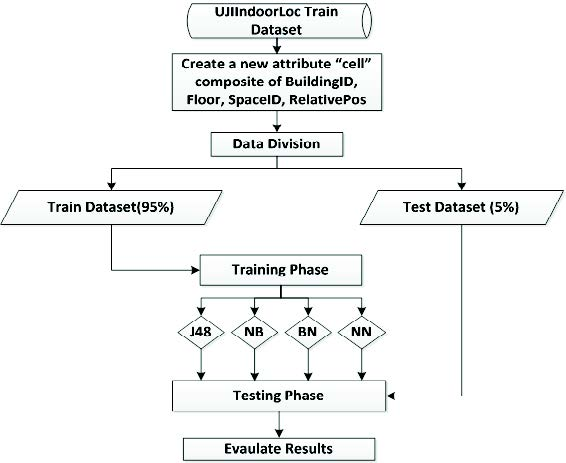
\includegraphics[scale=1]{figures/newattribute.jpg}
%		\caption{The new attribute “cell” construction phase}
%		\label{fig:newAttribute} %% NOTE: always label *after* caption!
%	\end{center}
%\end{figure}

%\todo{Compléter cette partie qui semble importante}
